\section{Minimum Cut Problem }
\paragraph{Input} a graph $G=(V,E,w), W: E \rightarrow \mathbb{R}^+[s\neq t, s,t, \in V]$

\paragraph{Output} a partition of V into S,T (T = V \ S) s.t.

\begin{itemize}
	\item[(i)] $S \neq \emptyset \land T \neq \emptyset [s \in S, t \in T]$
	\item[(ii)] $w(S,T) = \sum_{u\in S, v\in T}w(u,v)$ is minimum over all partitions
\end{itemize}
\begin{center}
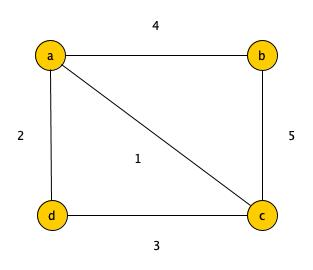
\includegraphics[scale=0.75]{img/graph7} \\
\end{center}
\begin{tabular}{|c|c|} \hline 
	$S$ & $w(S,T)$ \\ \hline 
	a & 7 \\
	b & 9 \\
	c & 9 \\
	\textbf{d} & \textbf{5} \\
	a,b & 8 \\
	b,c &  8 \\
	c,d &  8 \\
	d,a &  8 \\ \hline
\end{tabular} \\

(Max-Cut Problem is NP complete) 

\paragraph{Observation} MinCut $\stackrel{n^2}{\leq}$ Min(s-t)-Cut
$\rightarrow$ can we do better: $\mathcal{o}(n^2)$ \\

\begin{verbatim}
MinCut(G)
min <- infty
for each s in V 
    for each t in V: s != T // two fors -> n^2
        (S,T) <- Min-s-t-Cut(s,t)
        if(S,T) is lighter than min // in Term of weights
            min <- (S,T)
\end{verbatim}

Merging a and b in example \\
\begin{center}
	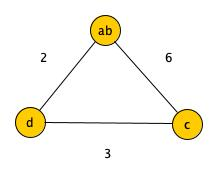
\includegraphics[scale=1]{img/graph8}
\end{center}

Edge ab - c is sum of weight (5 and 1)

\subsubsection{Operation: Merge of two verties}

Given a graph $G = (V,E,w)$ \& $s,t \in V$ , $s \neq t$ the Graph $G\ \{s,t\} = (V',E',w')$ obtained by merging $s,t$. \\

$$V' = V \ \{s,t\} \cup \{X_{s,t}\}$$

$$E' = E \ \{(u,v) \in E: u,v \in \{s,t\}\} \cup \{(X_{s,t},v): (s,v) \in E \lor (t,v) \in E\}$$

$$w'(X_{st},v) = \begin{cases}
w(s,v) & (s,v) \in E \& (t,v) \notin E \\
w(t,v) & (s,v) \notin E \& (t,v) \in  E \\
w(s,v) + w(t,v) & (s,v) \in E \& (t,v) \in E \\
0 & otherwise
\end{cases}$$

\subsection{Theorem 1}

Let $s,t \in V$ of a graph $G = (V,E)$ \& let $G \ \{s,t\}$ be the graph obtained by $G$ by merging $s$ \& $t$.

Then: 
$$min-cut(G) = min\{min-(s,t)-cut(G), minCut(G\ \{s,t\})\}$$


\paragraph{Proof} Let $(S,T)$ be a min cut of $G$ \\ 
$\Rightarrow {s,t} \in \lor \{s,t\} \in T$ [first part] \\
or \\
$s \in S$ \& $t \in T \lor t \in S$ \& $s \in T$ [second part]

\begin{flushright}
	$\square$
\end{flushright}



\begin{verbatim}
n = |V(G)|
if(n=2) return ({v1},{v2})
else let s,t in V, s != t
    (S,T) <- min-(s,t)-cut for G exists algorithm
    (S',T') <- MinGut(G \ {s,t}) // recursion
    return min{(S,T),(S',T')}
\end{verbatim}

Theorem 1 $\Rightarrow$ Correctnes \\

Complexity $\approx (n-1) \cdot c$, where $c$ min-(s,t)-cut(G) \\

\paragraph{Observation} in linear time reduceable $\mathcal{O}(n)$

\subsection{Min-(s,t)-Cur Problem (Stoer \& Wagner)}

\paragraph{Idea}
\begin{itemize}
	\item finds an ordering of the vertices $v_1,..,v_n$, $n = |V(G)|$: ($\{v_1,v_2,...v_{n-1}\},\{v_n\}$) is a min ($v_{n-1},v_n$)-cut
	\item Let $S_i = \{v_1,...,v_i\}$ starting from an arbitrary vertex $v_1$. Then $v_{i+1}$ is selected $s,t$. $w(v_{i+1},S_i) \geq w(v,S_i) \forall v\in V \ S_i$
\end{itemize}



\subsubsection{Example}
\begin{center}
	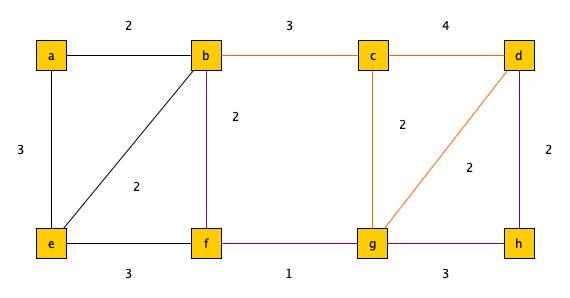
\includegraphics[scale=0.75]{img/graph9}
\end{center}
\begin{tabular}{|c|c|l|}\hline 
	$i$ & $v$ & $S$ \\ \hline 
	1 & b & b \\
	2 & c & b,c \\
	3 & d & b,c,d \\
	4 & g & b,c,d,g \\
	5 & h & b,c,d,g,h \\
	6 & f & b,c,d,g,h,f \\
	7 & e & b,c,d,g,h,f,e \\ \hline 
\end{tabular} \\
$\Rightarrow$ Stoer \& Wagner $(\{a\}, \{b,c,d,g,h,f,e\})$ must be a min (a,e)-cut.

\begin{verbatim}
MinCutPhase(G)
    v1 = any vertex of G
    S = {v1}
    for i = 2 ... n do
        vi <- w({bi},S) >= w({v}, S), v not in V \ S
        S = untion(S, {vi}) // ordered set
    return ({vn},{v1,...,n(n-1)})
\end{verbatim} 
$$\forall v \in V \ S: key(v) = \sum_{v'\in S}w(v,v')$$

$v_{i+1}$ in the vertex with max key

\subsubsection{Fibonacci Heaps}

$\mathcal{O}(Extract-Max) = \mathcal{O}(\log n)$ \\

UpdateKey = $\mathcal{O}(1)$ \\

in total: $|V| \times$ Extract Max and $|E| \times$ UpdateKey $\Rightarrow \mathcal{O}(|V| \log |V| + |E|)$


\subsection{Theroem 2}

$(T,s) = (\{v_1,...,v_{n-1}\}, \{v_n\})$ is a min ($v_{n-1}$, $v_n$)-cut

\paragraph{Proof}

Let $(S,T)$ be any ($v_{n-1},v_n$) cut. We prove: $$w(\{v_1,...mv_{n-1}\}, \{v_n\}) \leq w(S,T)$$
\begin{center}
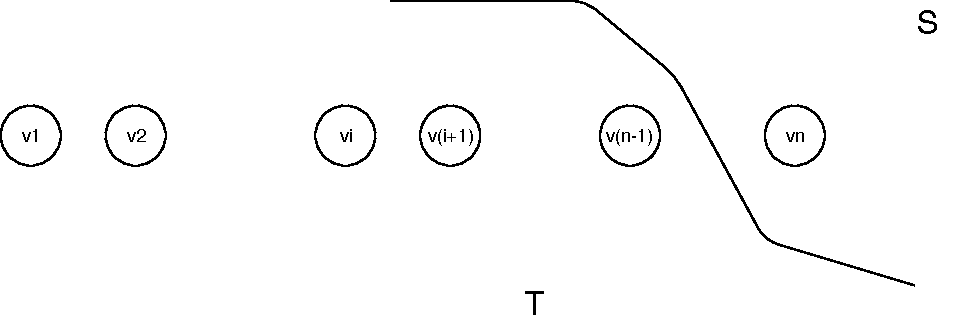
\includegraphics[scale=1]{img/cut}
\end{center}

Critical: $v_i$ is critical iff $\Leftrightarrow (v_i \in S \& v_{i-1} \in T)$ or ($v_i \in T \& v_{i-1} \in S) \Rightarrow v_n \in S \& v_{n-1} \in T$ \\

$A_i := w(\{v_1,..,v_{i-1}\}, \{v_i\}) \leq w(\{v_1,...,v_{i}\} \cap S, \{v_1,...,v_i\}\cap T) =: B_i$ \\

$\forall critical vertex v_i \Rightarrow $ Theorem is proved \\

By induction on the number of critical vertices
\begin{itemize}
\item for the critical vertiex $v_{i_0}:$ \\
\begin{center}
	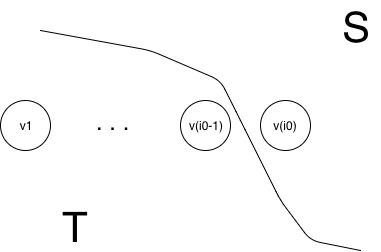
\includegraphics[scale=0.5]{img/cut2}
\end{center}
$\Rightarrow A_{i_0} \leq B_{i_0} \checkmark$  

\item  $A_i \leq B_i$ holds up to the critical vertex $v_i$ [Induction hypothesis]
\item  let $v_j$ be the next critical vertex
\begin{align*}
A_j &= w(\{v_1,...,v_{j-1}\}, \{v_j\}) \\
&= w(\{v_1,...,v_{i-1}\}, \{v_i\}) + w(\{v_1,...,v_{j-1}\}, \{v_j\}) \\
&\stackrel{Stoer+Wagner}{\leq} w(\{v_1,...,v_{i-1}\}, \{v_i\}) + w(\{v_1,...,v_{i-1}\}, \{v_i\}) \\
&\stackrel{IH}{\leq} w(\{v_1,...,v_i\}\cap S,\{v_1,...,v_i\} \cap T) + w(\{v_1,...,v_{j-1}\}, \{v_j\}) \\
&\leq w(\{v_1,...,v_j\}\cap S,\{v_1,...,v_j\}\cap T)
\end{align*}
\begin{flushright}
$\square$
\end{flushright}
\end{itemize}

\paragraph{Claim } 
$w(\{v_1,...,v_{j-1}\},\{v_j\}) \leq w(\{v_1,...,v_{j-1}\} \cap S, \{v_1,...,v_j\}\cap T)$

\paragraph{Proof}
\begin{align*}
w(\{v_1,...,v_{j-1}\},\{v_j\}) &= w(\{v_1,...,v_{i-1}\},\{v_j\}) + w(\{v_i,...,v_{j}\},\{v_j\}) \\
&\stackrel{Stoer+Wagner}{\leq} w(\{v_1,...,v_{i-1}\},\{v_i\}) + w(\{v_i,...,v_{j}\},\{v_j\}) \\
&\stackrel{I.H.}{\leq} w(\{v_1,...,v_{i}\} \cap S, \{v_1,...,v_i\}\cap T) + w(\{v_i,...,v_{j}\},\{v_j\}) \\
&\stackrel{\text{By the fact that vj is critical}}{\leq} w(\{v_1,...,v_{j}\} \cap S, \{v_1,...,v_j\}\cap T) 
\end{align*}

\paragraph{Code}
\begin{verbatim}
MinCut(G)
    n=|V(G)|
    if n = 2 return ({v1},{v2})
    else
        ({v1,...,v(n-1)}{vn}) <- MinCutPhase(G) // V logV+E (Stoer Wagner)
        (S,T) <- MinGut(G\{s,t}) // O(V) (first part in complexity)
        return the lighter of (S,T) and ({v1,...,v(n-1)}{vn})
\end{verbatim} 

\paragraph{Complexity} $\mathcal{O}(V(V \log V+E))$

\subsubsection{Example}

\begin{center}
	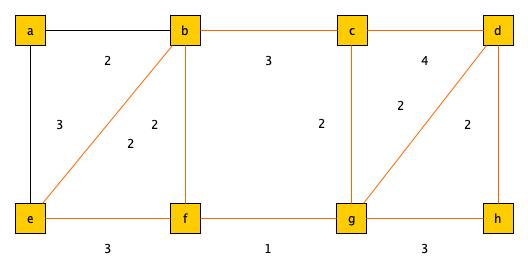
\includegraphics[scale=0.5]{img/graph4}
\end{center}

$v_1$ = b\\
$v_2$ = c\\
$v_3$ = d\\
$v_4$ = g \\
$v_5$ = h \\
$v_6$ = f \\
$v_7$ = e \\
--- \\
$v_8$ = a \\

$\Rightarrow w(\{v_1,...,v_7\},\{v_8\}) = 5$ \\

$\Rightarrow$ merge a and e

\begin{center}
	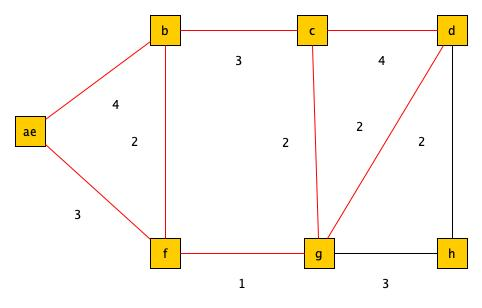
\includegraphics[scale=0.5]{img/graph3}
\end{center}

$v_1$ = b\\
$v_2$ = ae\\
$v_3$ = f\\
$v_4$ = c\\
$v_5$ = d  \\
---  \\
$v_6$ = g \\

$\Rightarrow w(\{v_1,v_2,...,v_6\},^\{v_7\}) = 5$ \\

$\Rightarrow$ merge h and g \\

go on like that.

\newpage
\section{The Max Flow problem}

\paragraph{Input} 
\begin{itemize}
\item  $A$ directed weighted graph (network) $D = (V,E,c)$
\item $c: E \rightarrow  \mathbb{R}^+$ capacity
\item $s,t \in V: s \neq t \& indegree(s) = 0 \& outdegree(t) = 0$
\item $s$: source, $t$: target
\end{itemize}
\begin{center}
	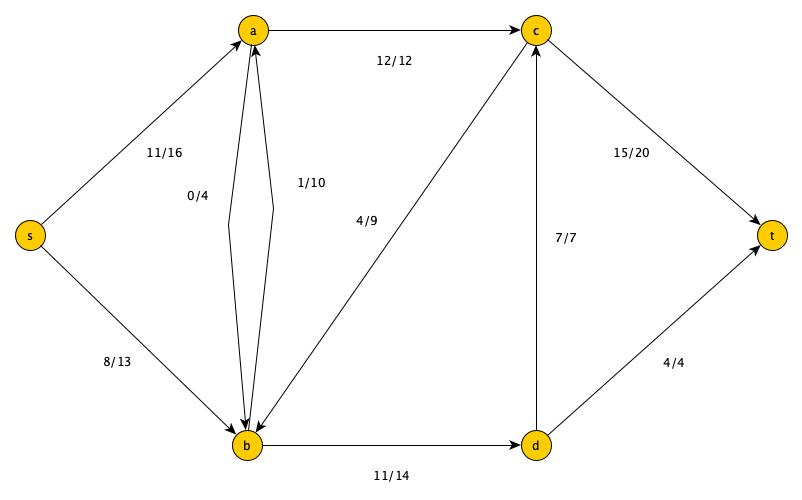
\includegraphics[scale=0.5]{img/graph5}
\end{center}
\textit{Syntax: x/y: x is the flow, y is capacity.} |f| = 19 \\
\textit{Informal: The max quantity of items that can be send from $s$ to $b$ without deviating the capacities \& without storing anything in between.}

\paragraph{Output}
$f: E \rightarrow \mathbb{R}^+$: flow function

\begin{itemize}
\item[(i)] $0 \leq f(u,v) \leq c(u,v) \forall (u,v) \in E$

\item[(ii)] $\sum_{(u,v)\in E}f(u,v) = \sum_{(v,u) \in E}f(v,u) \forall v  \in V \ \{s,t\}$

\item[(iii)] $\sum_{(s,v) \in E} f(s,v)$ is maximized $ (s,v)\in E$ over all flow functions

\end{itemize}

\begin{itemize}
	\item[(i)] called \textbf{capacity constraint}
	
	\item[(ii)] called \textbf{flow consertation}
	
	\item[(iii)] \textbf{called max flow} denoted by $|f^*|$
	
\end{itemize}

\fbox{\parbox{\linewidth}{inflow (flow coming in) and outflow (flow going out) on v}}

\subsection{Example}
\begin{center}
	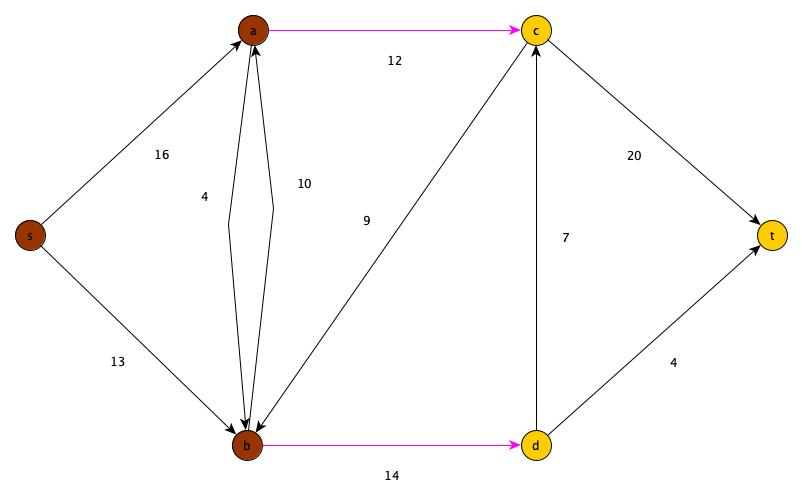
\includegraphics[scale=0.5]{img/graph6}
\end{center}

Cut brown (S) and yellow (T), so $c(S,T) = 26 (= 12+14)$ and
$|l| \leq  c(S,T) \forall  f $


\subsection{Lemma}

$$\forall \text{flow of D} \& \forall cut (S,T): s\in S \& t\in T: |f| \leq c(S,T)$$

\paragraph{Proof}
\begin{align*}
|f| &= \sum_{(s,v)\in E}f(s,v) - \sum_{(v,s)\in E}f(v,s) + \underbrace{\left( \sum_{(u,v)\in E; u\in S\ \{s\}}f(u,v) - \sum_{(u,v)\in E; u\in S\ \{s\}}f(v,u)\right)}_{\text{[0 by (ii)]}} \\
&= \sum_{u\in S} \left( \sum_{(u,v)\in E}f(u,v) - \sum_{(u,v)\in E}f(v,u) \right) \\
& =\underbrace{\left( \sum_{(u,v)\in E/u,v\in S}f(u,v) - \sum_{(u,v)\in E/u,v\in S}f(v,u) \right)}_{\text{[0 by (ii)]}} + \left( \sum_{(u,v)\in E/u\in S,v\in T}f(u,v) - \sum_{(u,v)\in E/u\in S,v\in T}f(v,u) \right) \\
&= \sum_{(u,v)\in E/u\in S,v\in T}f(u,v) - \underbrace{\sum_{(u,v)\in E/u\in S,v\in T}f(v,u)}_{\text{[this part $\geq$ 0 by (i) so cut out]}}
\\
&\leq \sum_{(u,v)\in E/u\in S,v\in T}f(u,v) \stackrel{(i)}{\leq} \sum_{(u,v)\in E/u\in S,v\in T}c(u,v) = c(S,T) 
\end{align*}


\subsection{Corolary 1}

$|f^*| \leq c(S,T) \forall (S,T)$ being an (s,t)-cut

\subsection{Corolary 2}
If there exists a flow f and (s,t)-cut (S,T):

$$|f| = c(S,T) = \sum_{(u,v)\in E,s\in S,v\in T}c(u,v)$$

$$\Rightarrow |f^*| = |f| it's optimal s\in S, v\in T$$


\subsection{Max-flow/min-cut Theorem:}

$$|f^*| is max \Leftrightarrow \exists (s,t)-cut (S,T): |f| = c(S,T)$$

\subsection{Augmenting Path}

$(s,t)$-Path in $D$ align which we can push flow (and augment the flow)

\begin{verbatim}
Ford-Fulkerson (G,s,t)
    initialize f to 0 
    While(esists augmenting path P from s to t)
        Augment f by the bottleneck of P
    return f
\end{verbatim}
\begin{center}
	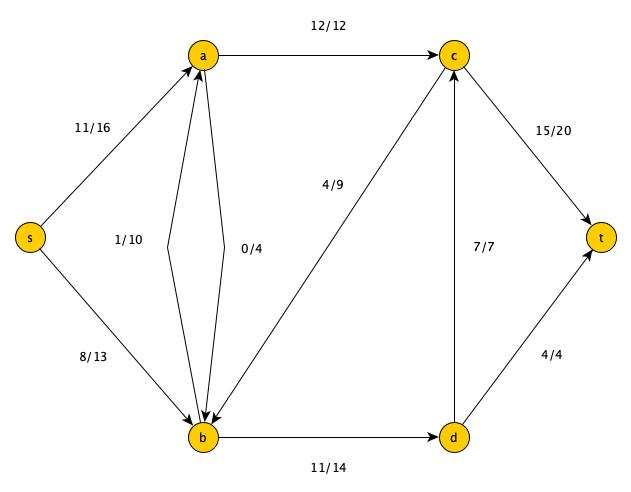
\includegraphics[scale=0.5]{img/graph10}
	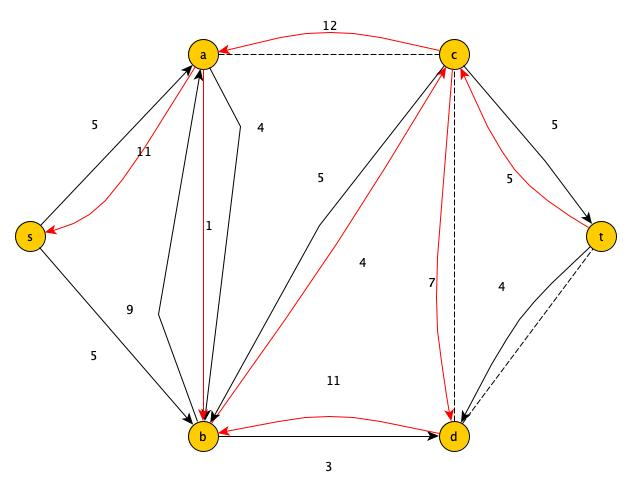
\includegraphics[scale=0.5]{img/graph11}
\end{center}

\subsection{Residual Network}
Describes for every edge $(u,v) \in $E the amount of flow that can be further pushed along $(u,v)$.

$$c_f = (V_f,E_f): 
V_f = V, 
E_f = \{(u,v): c_f(u,v) > 0\},$$$$ 
c_f \text{ residual capacity} \rightarrow 
c_f = \begin{cases} c(u,v)-f(u,v) & (u,v)\in E \\
f(v,u) & (v,u)\in E \\
0 & othehrwise
\end{cases}$$

\begin{center}
	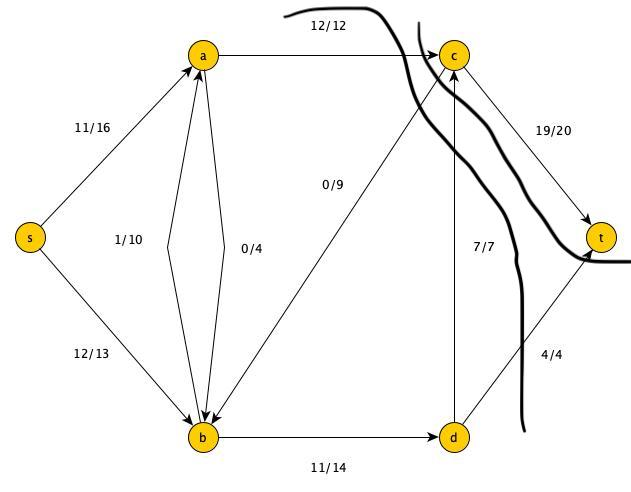
\includegraphics[scale=0.5]{img/graph12}
\end{center}
path: (s,b,c,t), $|f| = 24 > 19, c(S,T) = 24 \Rightarrow f $optimal 

\paragraph{Question} Is the algorithm correct? \\

Augmenting Path Theorem: \\

$f^* \text{ is max flow} \Leftrightarrow \nexists\text{ augmenting path in} G^*_f$ \\

Max-Flow Min-Cut Theorem: \\
$f^*$ is max flow $\Leftrightarrow \exists (s,t)-cut (S_0,T_0), |f^*| = c(S_0,T_0)$

\subsubsection{Theorem}
(i)(ii)(iii) are equivalent: \\
\begin{itemize}
	\item[(i)] $f^*$ is max flow
	
	\item[(ii)] $\nexists$ augmenting path in $G^*_f$
	
	\item[(iii)] $\exists (s,t)-cut (S_0,T_0)$: $|f^*| = c(S_0,T_0)$
	
\end{itemize}
(i) $\Rightarrow$ (ii)$\Leftrightarrow$ $\neg$ (ii) $\Rightarrow \neg$(i) \\
$\neg$(ii) $\Rightarrow \exists$ aug. path $\Rightarrow$ aug. the path $\Rightarrow f^*$ was not max
\begin{flushright}
$\square$
\end{flushright}
(ii) $\Rightarrow$ (iii) \\

\paragraph{Example}
\begin{center}
	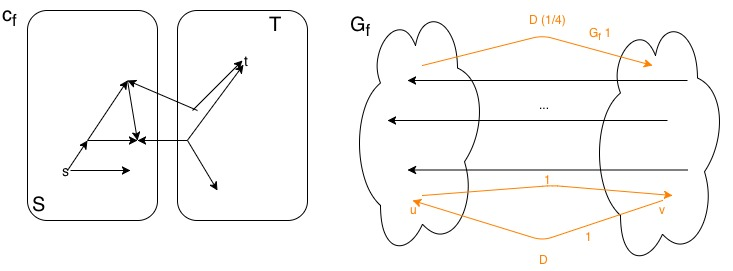
\includegraphics[scale=0.5]{img/graph13}
\end{center}
S: vertices that are reachable by s in $G_f$ \\
T = $V$\ S \\
(ii) $\Rightarrow T \neq  \emptyset (t\in T), (S \neq \emptyset, T \neq \emptyset)$ \\
$|f^*| = ... = \sum_{u,v\in E, u,v\in S}f(u,v)-\sum_{u,v\in E, v,u\in S}f(v,u) + \sum_{u,v\in E, u\in S,v\in T}f(u,v)-\sum_{u,v\in E, u\in S,v\in T}f(v,u)$ \\
$G_p$ s.a. \\
if$(u,v)\in E$ $\Rightarrow f(u,v) = c(u,v)$  full \\
if$(v,u)\in E \Rightarrow f(u,v) = 0$ empty
\begin{flushright}
	$\square$
\end{flushright}

(iii) $\Rightarrow$ (i) \\
see last lecture, follows from the fact that 
$$\forall f \forall (s,t)-cut (S,T): |f| \leq c(S,T)$$

\fbox{\parbox{\linewidth}{If capacities are integers, then $|f^*|$ is also an integer \\ theorem (iii) $|f^*|$ is sum of integers}}



\begin{verbatim}
FordFulkerson(D,s,t)
    for each edge (u,v)\in E // O(|E|)
        f[u,v] <- 0
        flow[u,v] <- 0
    compute G_f // O(|V|+|E|)
    While(exists aug path P from s to t in G_f) // P * O(|E|) oder so aehnlich
        x = min{c_f(u,v): (u,v) in P}
        for earch edge (u,v) in P # O(|E|)
            if(u,v) in E f[u,v] = f[u,v] + x
            if(v,u) in E f[v,u] = f[v,u] - x
            update G_f // O(|V|)
\end{verbatim}

\fbox{\parbox{\linewidth}{if capacities are not integers, then FordFulkersion algorithm may not terminate \\
Assumption: all capacities are integers $\Rightarrow |f^*|$ is integer}}

At each interation the flow is augmenting by at least 1 unit (the augmenting path goes through an edge (u,v): $c_f(u,v)=1$)\\
$\Rightarrow$ While-loop terminates after $|f^*|$ steps \\
$\Rightarrow$ Complexity: $\mathcal{O}(|f^*|\cdot |E|)$ \\

\fbox{\parbox{\linewidth}{1. $\mathcal{O}(|f^*| \cdot |E|)$ depends on the size of the output \\
2. $\exists$ instances that require $\mathcal{O}(|f^*|\cdot |E|)$}} 


\begin{center}
	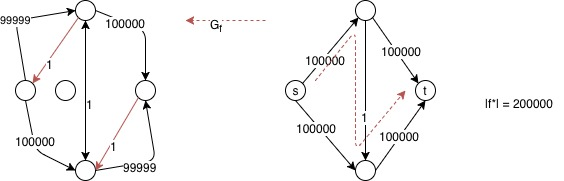
\includegraphics[scale=0.5]{img/graph14}
\end{center}

Can't pass more then max flow on edge. So on more paths the sum still has to be smaller than the max flow on each edge. To calculate max flow efficiently you need to find the min cut. 
\paragraph{Idea} Choose a path from s to t. So how much flow can be passed through that path? $\Rightarrow$ smallest max flow on an individual edge on the path. Push this amount through the path. (At least on edge (with the smallest max flow) is now full). So it translates to the following graph with the capacities $ (u,v) \Rightarrow c(u,v)-f(u,v)$. Non existing edges have capacity 0 and get - the flow the edge in the other direction has. (red in graph): 
\begin{center}
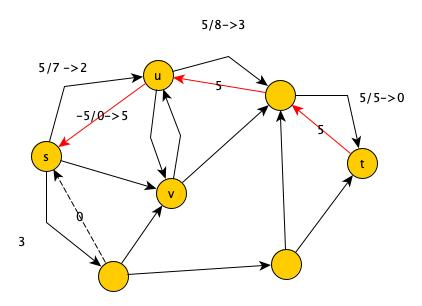
\includegraphics[scale=0.5]{img/graph15} 
\end{center}
Continue with other paths. With the backwards edges the algorithm can tell that the push over this edge was a bad decision by wanting to push over this edge. So we leave the algorithm the freedom to backtrack. \\
Maximum complexity: $\mathcal{O}(|E|\cdot f^*)$. 
\subsection{EdmondKarp}
Search for the shortest path in the Graph ($\#edges$). Augmenting path $s$ to $t$ is the shortest from $s$ to $t$. $\Delta_f(v)$ = min number of edges in $G_f$ from $s$ to $v$. We only need to prove the complexity. (Correctness follows from \texttt{FordFulkerson}) \\
$\mathcal{O}(|V|\cdot |E|^2)$ complexity on \texttt{EdmondKarp}. Wen want to prove that we have $\mathcal{O}(|V|\cdot |E|)$ steps (cause shortest path is $\mathcal{O}(|E|)$.
\paragraph{Proof} At each step there is a bottleneck edge. We want to show that every edge becomes bottleneck once. Because we have more than $|E|$ steps some need to be bottleneck twice. So we prove: \\
$$\forall (u,v): (u,v) \text{ is a BN at most }\mathcal{O}(|V|)\text{ times}$$
We need to state on more property: One edge on the residual network goes to zero (bottleneck). $\Delta_f(w) = |\text{shortest path from s to w in }G_f|$ By changing flow (with the algorithm) we change the network (add and drop edges). By adding an edge there may be a shorter path from $s$ to $w$. \\
We have flow $f$ and after a step we have $f'$ with $\forall w: \Delta_f(w) \leq \Delta_{f'}(w)$. We will prove this first by looking at the contradiction: $\Delta_f(w) > \Delta_{f'}(w)$. 
\begin{itemize}
\item[A:] $\Delta_f(w) > \Delta_{f'}(w) $ [Hy] 
\end{itemize}
$\underbrace{s-...-u-w}_{\text{shortest path}}$ 
\begin{itemize}
\item[B:] $\Delta_f(u) = \Delta_f(w)-1$ 
\item[C:] $\Delta_f(u) \leq \Delta_{f'}(u)$
\end{itemize}
So:
$$\Delta_f(w) = \Delta_f(u)+1 \leq \Delta_{f'}(u)+1 = \Delta_{f'}(w) \Leftrightarrow \Delta_f(w) \leq \Delta_{f'}(w) \; \lightning \text{to [Hy]}$$
So now we know $\Delta_f(w) \leq \Delta_{f'}(w)$. So now we prove 
$$\forall (u,v): (u,v) \text{ is a BN at most }\mathcal{O}(|V|)\text{ times}$$
We can say $\Delta_f(w) \leq |V|$, so $|V|$ is the upper bound.  We have a network with a bottleneck path. At step $i$ the edge $(u,w)$ is the bottleneck so it doesn't exist in step $i+1$. But it exists from $w$ to $u$. On step $j$ it can become bottleneck again but there has to be a step $k$ between $i+1$ and $j$ where the edge $(w,u)$ needs to be bottleneck ($\Rightarrow$ on the shortest path from s to t). So we have the shortest paths: 
$$(i): s-...-u-w-...-t \Rightarrow \Delta_{f_i}(u) = \Delta_{f_i}(w)-1 $$ 
$$(k): s-...-w-u-...-t \Rightarrow \Delta_{f_k}(u) = \Delta_{f_k}(w)+1 $$ 
$$\Delta_{f_i}(w) \leq \Delta_{f_k}(w)$$
$$\Delta_{f_i}(u) = \Delta_{f_i}(w)-1 \leq \Delta_{f_k}(w)-1 = \Delta _{f_k}(u)-1-1$$
Augmentation of at least -2. \\
Because of the upper bound an edge can be bottleneck not more than $\frac{|V|}{2}$ times. $\Rightarrow \mathcal{O}(\frac{|V|}{2} \cdot |E|)$ \\
$\Rightarrow \mathcal{O}(|V| \cdot |E|^2)$ complexity.
\begin{flushright}
	$\square$
\end{flushright}

$|E|$ can me much larger than $|V|$. There is an algorithm that solves Max-Flow in $\mathcal{O}(|V|^2 \cdot |E|)$: \texttt{PUSH-RELABEL} or \texttt{TARJAN-GOLDBERG}. There exist also implementations where you have $\mathcal{O}(|V|^3)$ or $\mathcal{O}(|V|^2\cdot \sqrt{|E|})$. \\
Residual Network is same to EdomdKarp. Difference: you try to do things ore local. On EdmondKarp you always search from $s$ to $t$ $\Rightarrow |E|^2$. \\
Locally you don't know if the flow will reach $t$, so the vertex tries to push the flow to following vertices. If you are lucky this system brings as much flow as possible to $t$. \\
Each vertex has a label, that may change while the algorithm runs (\texttt{relabel}). $s$ will have label $|v|$ and $t$ label $|0|$ all the time. With the algorithm the other labels can change. A vertex can push flow to other vertices if
\begin{enumerate}
	\item There is an edge where you can push (with residual capacity)
	\item The vertex that pushes has a higher label than the vertex that is receiving.
\end{enumerate}
Each step we take one vertex and try to push. So you push to a vertex with lower label and update the capacity on this edge. This you do edge by edge. It can appear that a vertex needs to push flow but has only edges to vertices with higher labels. So the flow gets stuck. So you relabel: You look at the vertices that the vertex could push to and increase the pushing vertex-label to $min(\text{neighbours labels})+1$. You start with every label (except $s$) 0. Then you start pushing from $s$. You won't be able to push more flow than the outgoing capacities on $s$. That is the first upper bound. If somewhere you get stuck and can't go on, try to push it a little bit back. \\
It could happen that $s$ can push as much flow as all the outgoing capacities. So all neighbours of $s$ are now "active". All these vertices has label 0 now. That means they can't push. Relabel one of them to 1. This one tries now to send his received flow. Maybe it has not enough outgoing capacity, so there will be some flow stuck un this vertex, but you don't need to push it back, because $s$ has no capacity left. So the vertex stays active. At some point you give that vertex the label $|v|+1$ to send the flow, that is too much, back to $s$ to say $s$ that this is too much. That happens at the closing part of the algorithm.

\subsection{Matching}
\begin{center}
	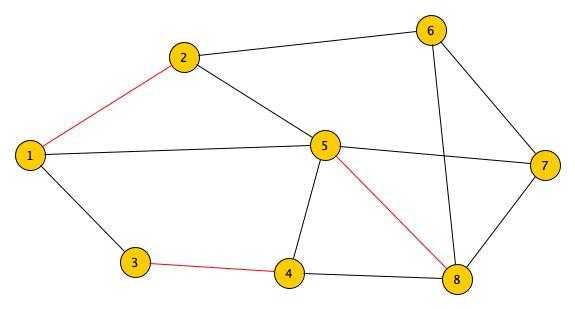
\includegraphics[scale=0.5]{img/graph16}
\end{center}
\paragraph{Matching} On the chosen set of edges there is no common vertex (equivalent to independent set on vertices).
\paragraph{Maximal Matching} There is no edge that can be added without violating the matching constraint. So on the example above only edge $(6,7)$ could be added to get the maximum matching. 
\paragraph{Maximum Matching} The maximum of the maximal matchings. \\
The concept of Max Flow and Maximum Matching is the same. \\
Don't go greedy on Maximum Matching. Usually you want the get the Maximum Matching. \\
We want to find the Maximum Matching in a bipartite graph. Give every edge the capacity 1. Add $s$ at one side with edge (1) to every vertex on that side and equivalent $t$ to the other side. SO at least one edge per vertex on the connecting edges can be taken. SO you search the maximum flow in the graph.
\begin{center}
	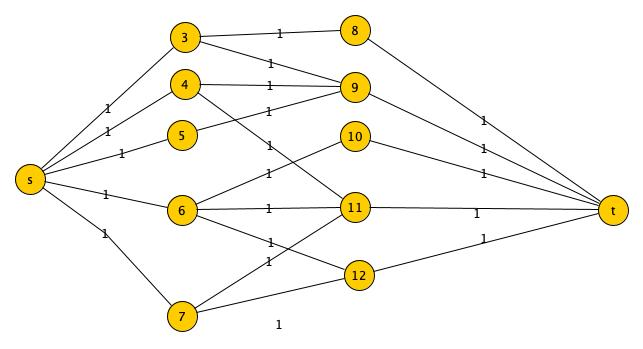
\includegraphics[scale=0.5]{img/graph17}
\end{center}
So to proof:
\begin{enumerate}
	\item If a flow $|f^*|$ exists $\Rightarrow$ matching exists
	\item a max matching exists $\Rightarrow$ a flow $|f^*|$ exists.
\end{enumerate}